\documentclass[12pt]{article}
\usepackage[spanish]{babel}
\usepackage{url}
\usepackage[utf8x]{inputenc}
\usepackage{amsmath}
\usepackage{graphicx}
\graphicspath{{images/}}
\usepackage{parskip}
\usepackage{fancyhdr}
\usepackage{vmargin}
\setmarginsrb{3 cm}{2.5 cm}{3 cm}{2.5 cm}{1 cm}{1.5 cm}{1 cm}{1.5 cm}

\title{Decide Ortosia - Autenticación}								%Title
								% Author
\date{12 Sept 2015}											% Date

\makeatletter
\let\thetitle\@title
\let\theauthor\@author
\let\thedate\@date
\makeatother

\pagestyle{fancy}
\fancyhf{}
\rhead{\theauthor}
\lhead{\thetitle}
\cfoot{\thepage}

\begin{document}

%%%%%%%%%%%%%%%%%%%%%%%%%%%%%%%%%%%%%%%%%%%%%%%%%%%%%%%%%%%%%%%%%%%%%%%%%%%%%%%%%%%%%%%%%

\begin{titlepage}
	\centering
    \vspace*{0.5 cm}
    
\includegraphics[scale = 0.2]{logo.png}\\[1.0 cm]	% University Logo
    \textsc{\LARGE Escuela Técnica Superior de Ingeniería  \newline\newline Informática}\\[2.0 cm]	% University Name
	\textsc{\Large Opera Id:125}\\[0.5 cm]				% Course Code
	\rule{\linewidth}{0.2 mm} \\[0.4 cm]
	{ \huge \bfseries \thetitle}\\
	\rule{\linewidth}{0.2 mm} \\[1.5 cm]
	
	\begin{minipage}{0.4\textwidth}
		\begin{flushleft} \large
			\emph{Autores:}\\
			Álvaro González \\		
			Luca Bonacini\\
            Antonio Millan \\
            Rodrigo Rojas \\
            Antonio Romero \\
			\end{flushleft}
			\end{minipage}~
			\begin{minipage}{0.4\textwidth}
            
			\begin{flushright} \large
			\emph{Tutores:} \\
			David Benavides Cuevas\\
            \emph{Opera Id: }
            125\\
			\emph{Grupo: }            
            G1\\
            
            
		\end{flushright}
        
	\end{minipage}\\[2 cm]
	
	
    
    
    
    
	
\end{titlepage}

%%%%%%%%%%%%%%%%%%%%%%%%%%%%%%%%%%%%%%%%%%%%%%%%%%%%%%%%%%%%%%%%%%%%%%%%%%%%%%%%%%%%%%%%%

\tableofcontents
\pagebreak

%%%%%%%%%%%%%%%%%%%%%%%%%%%%%%%%%%%%%%%%%%%%%%%%%%%%%%%%%%%%%%%%%%%%%%%%%%%%%%%%%%%%%%%%%

\section{Resumen}
Decide es una herramienta Open Source que se desarrolla con el fin de facilitar el voto online de manera segura, anonima y eficaz. Decide es un software heredado realizado por el equpo de Wadobo \url{https://github.com/wadobo/decide}.
En un primer momento se realizó un fork de este sistema para que podamos trabajar de forma aislada sin tener que modificar el sistema original.
El sistema se divide en varios subsistemas para facilitar el escalado y el mantenimiento del software. Dichos subsistemas se comunican entre ellos a través de llamadas REST.  


Nuestro grupo se encarga del subsistema de autenticación. Es el primer paso  para que un usuario pueda votar, garantizar que la persona que va a realizar el voto es quien dice ser. Como se ha comentado previamente el codigo fuente es heredado por lo que teniamos que seguir el lenguaje, estrategia y estructura que se había definido en un principio. El equipo decidió no desarrollar el subsistema con otra tecnologia ya que podría afectar al buen funcionamiento del sistema y podríamos encontrarnos con conflictos con los resto de subsistemas.  


Despues el equipo llego a un acuerdo sobre las tareas que se iban a desarrollar a lo largo del proyecto entre los que se encuentran distintos métodos de autenticación, documentación de la API, interfaz de usuario, etc. Cada miembro del equipo tenia asignadas unas tareas (\emph{issues}) y para gestionar el codigo se ha usado un repositorio GIT con el fin de que tuvieramos siempre la última versión del sistema (tanto por nuestra parte como con el resto de los equipos) y poder resolver conflictos de una forma mas eficiente.



\newpage	
\section{Introducción y contexto}

Es un proyecto para que el equipo de trabajo ponga en práctica y observe cómo se ponen en funcionamiento un proyecto real, en este caso se trabaja con Decide que es una plataforma didáctica de votación electrónica.

En el proyecto definimos diferentes subsistemas que serán más o menos independientes entre sí y que se interconectan implementando una API concreta.
Cada subsistema se encarga de una tarea concreta en el sistema de voto. Los subsistemas a realizar son los siguientes \cite{decide-subsistemas}

 \begin{enumerate}
    \item Autenticación
    \item Censo
    \item Votaciones
    \item Cabina de votación
    \item Almacenamiento de votos (cifrados)
    \item Recuento/ MixNet
    \item Post-procesado
    \item Visualización de resultados
 \end{enumerate}

Nuestro equipo se encargará del subsistema de autenticación que consistirá en autenticar al votante (con esto nos referimos a que se verifique que realmente la persona que vota dice ser quién es sin que se de el caso de suplantación de identidad), y que el votante solo pueda votar una vez en esa votación.

\section{Descripción del sistema}

\section{Planificación del proyecto}
Para la planificación del proyecto el equipo tuvo una reunión al principio del milestone para discutir y llegar a un acuerdo en las tareas que se iba a realizar durante el desarrollo del mismo. Las tareas estan definidas en el apartado de issues del repositorio \url{https://github.com/pablotabares/decide/issues} cada tarea tiene asignada una/s persona/s que seran los repsonsables de que dicha tarea se lleve a cabo en tiempo y en forma. 

Para gestionar el tiempo que ha dedicado cada miembro del equipo hemos utilizado la herramienta Toggle \cite{toggl} y se han incluido los reportes en el diario del equipo. 

Debido a que uno de los miembros se encuentra fuera de Sevilla y debe trabajar de forma remota el equipo llego a un acuerdo de reunirse los miercoles para conocer los avances y problemas que ha tenido el proyecto. Además se usaría Telegram \cite{telegram} como herramienta de comunicación de forma diaria.

\section{Entorno de desarrollo}

\section{Gestión del cambio, incidencias y depuración}

Las incidencias y cambios en el sistema se deben publicar en el apartado de  \emph{issues} en el repositorio del proyecto. Ya que estamos trabajando con otros subsistemas y otros equipos se propone que el titulo de la incidencia debería comenzar con Auth seguido de la incidencia o cambio propuesto. Por ejemplo: Auth - Email authentication \cite{auth-issue}

Además se debe indicar la persona responsable, una etiqueta, proyecto asociado y si es posible indicar el milestone como se muestra en la siguiente imagen:

\begin{figure}[h]
\centering
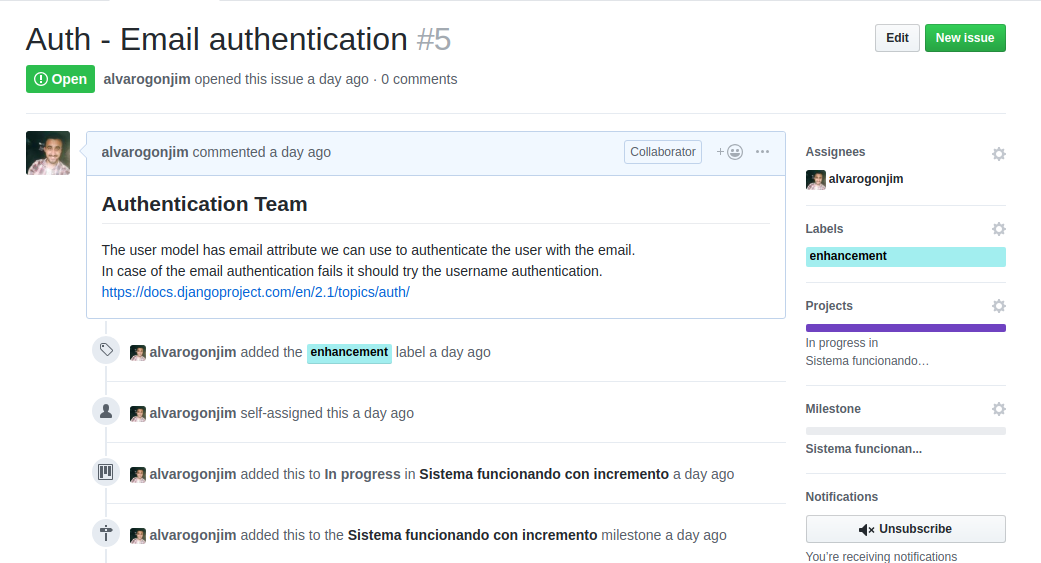
\includegraphics[width=1\textwidth]{issue-example.png}
\caption{Ejemplo de incidencia}
\end{figure}

\subsection{Gestión del código fuente}
La gestión del código fuente de nuestro proyecto se hará a través de Git ya sea por comandos (en la terminal) o a través de una interfaz de usuario. 
Los commits deben seguir la siguiente estructura \cite{commit-structure}:

Titulo: Extracto de los cambios en 50 caracteres o menos.

Texto explicativo más detallado, solo si es necesario. La línea en blanco que separa el titulo del resto del texto es crucial.
En el pie, se pueden poner referencias (ids) de las incidencias.

\begin{figure}[h]
\centering
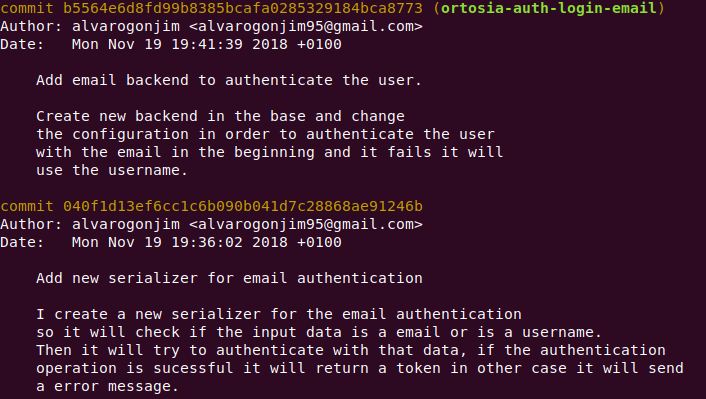
\includegraphics[width=0.8\textwidth]{commits.png}
\caption{Ejemplo de estructuras de commits}
\end{figure}


Para la gestión de ramas se empleará una rama por incidencia (aunque la incidencia sea muy leve o facil de realizar). El estructura de la rama debe ser ortosia-auth-\emph{titulo de la incidencia} como por ejemplo se puede ver en la imagen previa \emph{ortosia-auth-login-email}

Una vez que se haya finalizado el desarrollo de la incidencia se debe realizar un \emph{Pull Request (PR)} a la rama ortosia-auth. Este PR debe ser revisado por una/s persona/s que no sean los responsables y/o desarrolladores de la incidencia.

Cuando la rama base de nuestro equipo (ortosia-auth) sea estable y no tenga  fallos ni conflictos se realizará un PR a la rama master y posteriormente el proceso de despligue. 

\subsection{Gestión de la construcción e integración continua}
\subsection{Gestión de liberaciones, despliegue y entregas}

\section{Mapa de herramientas}
\section{Ejercicio de propuesta de cambio}
\section{Conclusiones y trabajo futuro}

\newpage	


\begin{thebibliography}{9}
\bibitem{decide-subsistemas} 
Dani GM
\textit
{https://github.com/EGCETSII/decide/blob/master/doc/subsistemas.md}

\bibitem{toggl} 
\textit{https://toggl.com/}

\bibitem{telegram} 
\textit{https://web.telegram.org/}

\bibitem{github-student} 
\textit{https://education.github.com/pack}

\bibitem{auth-issue} 
\textit{https://github.com/pablotabares/decide/issues/5}


\bibitem{commit-structure}
Miguel Angel Bueno Ferrer, 23 Abril 2017. 
\textit{https://blog.kirei.io/}
\end{thebibliography}

\end{document}